\section{Introduction}
%\introTips % Delete when no longer needed

Quantum algorithms show potential for speeding up computational routines, such
as the quantum Fourier transform \cite{shor1994algorithms}, simulating quantum systems \cite{lloyd1996universal, berry2015simulating, berry2015hamiltonian,  low2017optimal, low2019hamiltonian}, and solving linear systems
\cite{PhysRevLett.103.150502, wossnig2018quantum}. In
addition, quantum machine learning has demonstrated potential to advance
protein design and structure prediction, which can mitigate crises in resource
management, healthcare, and sustainability \cite{outeiral2021prospects,batra2021quantum,ajagekar2022new,andersson2022quantum}. Encoding chemical data onto quantum computers is a crucial first step in leveraging their potential because it enables the quantum system to directly manipulate and analyze data reflecting the underlying properties of the molecules themselves. This alignment between the nature of the data and the computer's processing capabilities can allow more natural and efficient simulations of complex chemical systems and can promote the application of downstream machine learning tasks with quantum computers \cite{doga2024perspective}. The quantum state preparation (QSP)
subroutine, which encodes classical data onto the amplitudes of a multi-qubit
quantum state, is an essential but often expensive step in such quantum algorithms and machine learning applications \cite{aaronson2015read}. 
Accurate encoding ensures that quantum algorithms can effectively model interactions between system components and potentially lead to performance improvements by allowing quantum computers to operate in a domain where their computational advantages are most pronounced \cite{pal2024quantum}. This foundation is essential for developing quantum algorithms that can exploit these advantages to solve problems like learning from chemical data like proteins to realize goals like capturing structure-property relationships. 

Efficient encoding of chemical data with good state preparation methods is critical for tasks such as quantum machine learning (QML) in cheminformatics that impact both the performance and the feasibility of these applications \cite{bernal2022perspectives, ajagekar2022new}. This initial step significantly influences the quality of insights derived from quantum machine learning such as pattern recognition in protein data or predictive modeling of their chemical interactions. Furthermore, efficient state preparation reduces the computational overhead associated with initiating QML tasks \cite{gujju2024quantum}. This can be caused by short coherence times and noisy quantum gate operations in current quantum 
hardware which limits the number of gates that can
be applied \cite{preskill2018quantum}. Therefore, executing quantum algorithms on near-term quantum
computers requires an efficient QSP implementation \cite{aaronson2015read}. By minimizing the time and gate circuit complexity needed for state preparation, the overall efficiency of quantum computations can be improved, allowing QML algorithms to perform complex tasks before the system becomes decoherent. This efficiency is particularly crucial in cheminformatics where the data types like protein representations are large and models are complex \cite{xu2020deep}. Effective state preparation thereby not only enhances the precision of the computations but also makes it feasible to apply quantum computing to real-world problems involving large-scale protein data.

We thus propose a framework for efficiently encoding chemical data like proteins as quantum states, as shown in Figure \ref{fig1}. The proposed approach comprises of three primary components: protein data as chemical input, quantum sparse state preparation circuits, and classical heuristic search methods, which operate in synergy to facilitate the encoding process. Protein data which includes the information on amino acid sequences and molecular properties provide the raw data that is necessary for quantum encoding. A core component of the proposed framework is the application of quantum circuits capable of preparing sparse quantum state preparation. Sparse quantum states on $n$ qubits have at most
$m$ nonzero amplitudes, where $m \ll 2^n$ \cite{PhysRevA.106.022617}. The efficient preparation of sparse 
quantum states finds applications in solving linear systems 
\cite{PhysRevLett.103.150502}, the quantum Byzantine agreement
\cite{10.1145/1060590.1060662}, and other quantum algorithms \cite{9272350, biamonte2017quantum}.  These circuits for quantum sparse state preparation are essential for effectively translating the high-dimensional and typically sparse chemical data into quantum information. The quantum circuits must be tailored to handle the specific properties of the protein data such as their amino acid constituents enabling a direct mapping of this data into quantum states. The third key element involves a classical heuristic search method to identify the optimal quantum gate sequence and parameters. These methods function as the feedback mechanism of the framework where classical computing techniques are utilized to refine and optimize the inputs and processes of the quantum circuits. This iterative process is vital for adjusting the encoding strategies based on the outcomes from quantum computations which enhances the efficiency and accuracy of the data encoding into quantum states.

Realizing the framework for efficient QSP implementation of protein data requires addressing a few research challenges revolving around mitigating the cost of a 
quantum circuit. Most commonly, quantum circuit cost is measured using
gate count or circuit depth \cite{1629135}. Gate count is the number of 
two-qubit gates in the quantum circuit. Single-qubit gates are ignored because 
they execute faster and introduce an order of magnitude less noise 
\cite{1629135}. Most quantum algorithms use the control-NOT (CX) gate as their 
two-qubit gate \cite{PhysRevLett.103.150502, 1629135, zhang2020toward, divincenzo1995two}. 
By contrast, circuit depth is the longest sub-sequence of non-commutative gates 
in the circuit \cite{1629135}. The greater the circuit depth, the longer the 
circuit takes to execute, leading to more noise from qubit decoherence \cite{10044235}. Several exact methods for QSP have been previously proposed like the uniformly controlled gates (UCG) approach \cite{1629135} and its various improvements \cite{bergholm2005quantum, PhysRevA.83.032302, 10044235, zhang2022quantum}. All of these algorithms return
asymptotically optimal gate counts within reasonable computation time.
However, asymptotically optimal is still exponential with number of 
qubits and such large gate counts cannot be feasibly implemented on near-term 
quantum computers. Many sparse state preparation methods have also been investigated \cite{10.1109/DAC18074.2021.9586240, Malvetti2021quantumcircuits}, however, they generally assume that CX gates can be applied to any qubit pair. As many quantum architectures follow a linear nearest neighbor (LNN) architecture wherein the $i$th qubit's nearest neighbors 
are the $i - 1$'th and $i + 1$'th qubit 
\cite{bravyi2022future, 
Saeedi_Wille_Drechsler_2010}, adaptability of protein encoded quantum state preparation for LNN should be ensured. 
An alternative to exact QSP methods is approximate encoding using
variational quantum circuits (VQCs) \cite{PhysRevResearch.4.023136, PhysRevA.98.032309}, which is hardware-adaptive and requires fewer CX gates compared to the exact QSP approach. Extracting optimal gate parameters for VQCs can be plagued by the barren plateau problem caused by vanishing gradients \cite{ rivera2021avoiding, PhysRevResearch.4.023136}. While exact quantum state preparation methods tend to use larger gate counts
compared to VQC-based methods, VQC-based methods require more computational
resources to generate a gate sequence.


\begin{figure}[h]
\centering
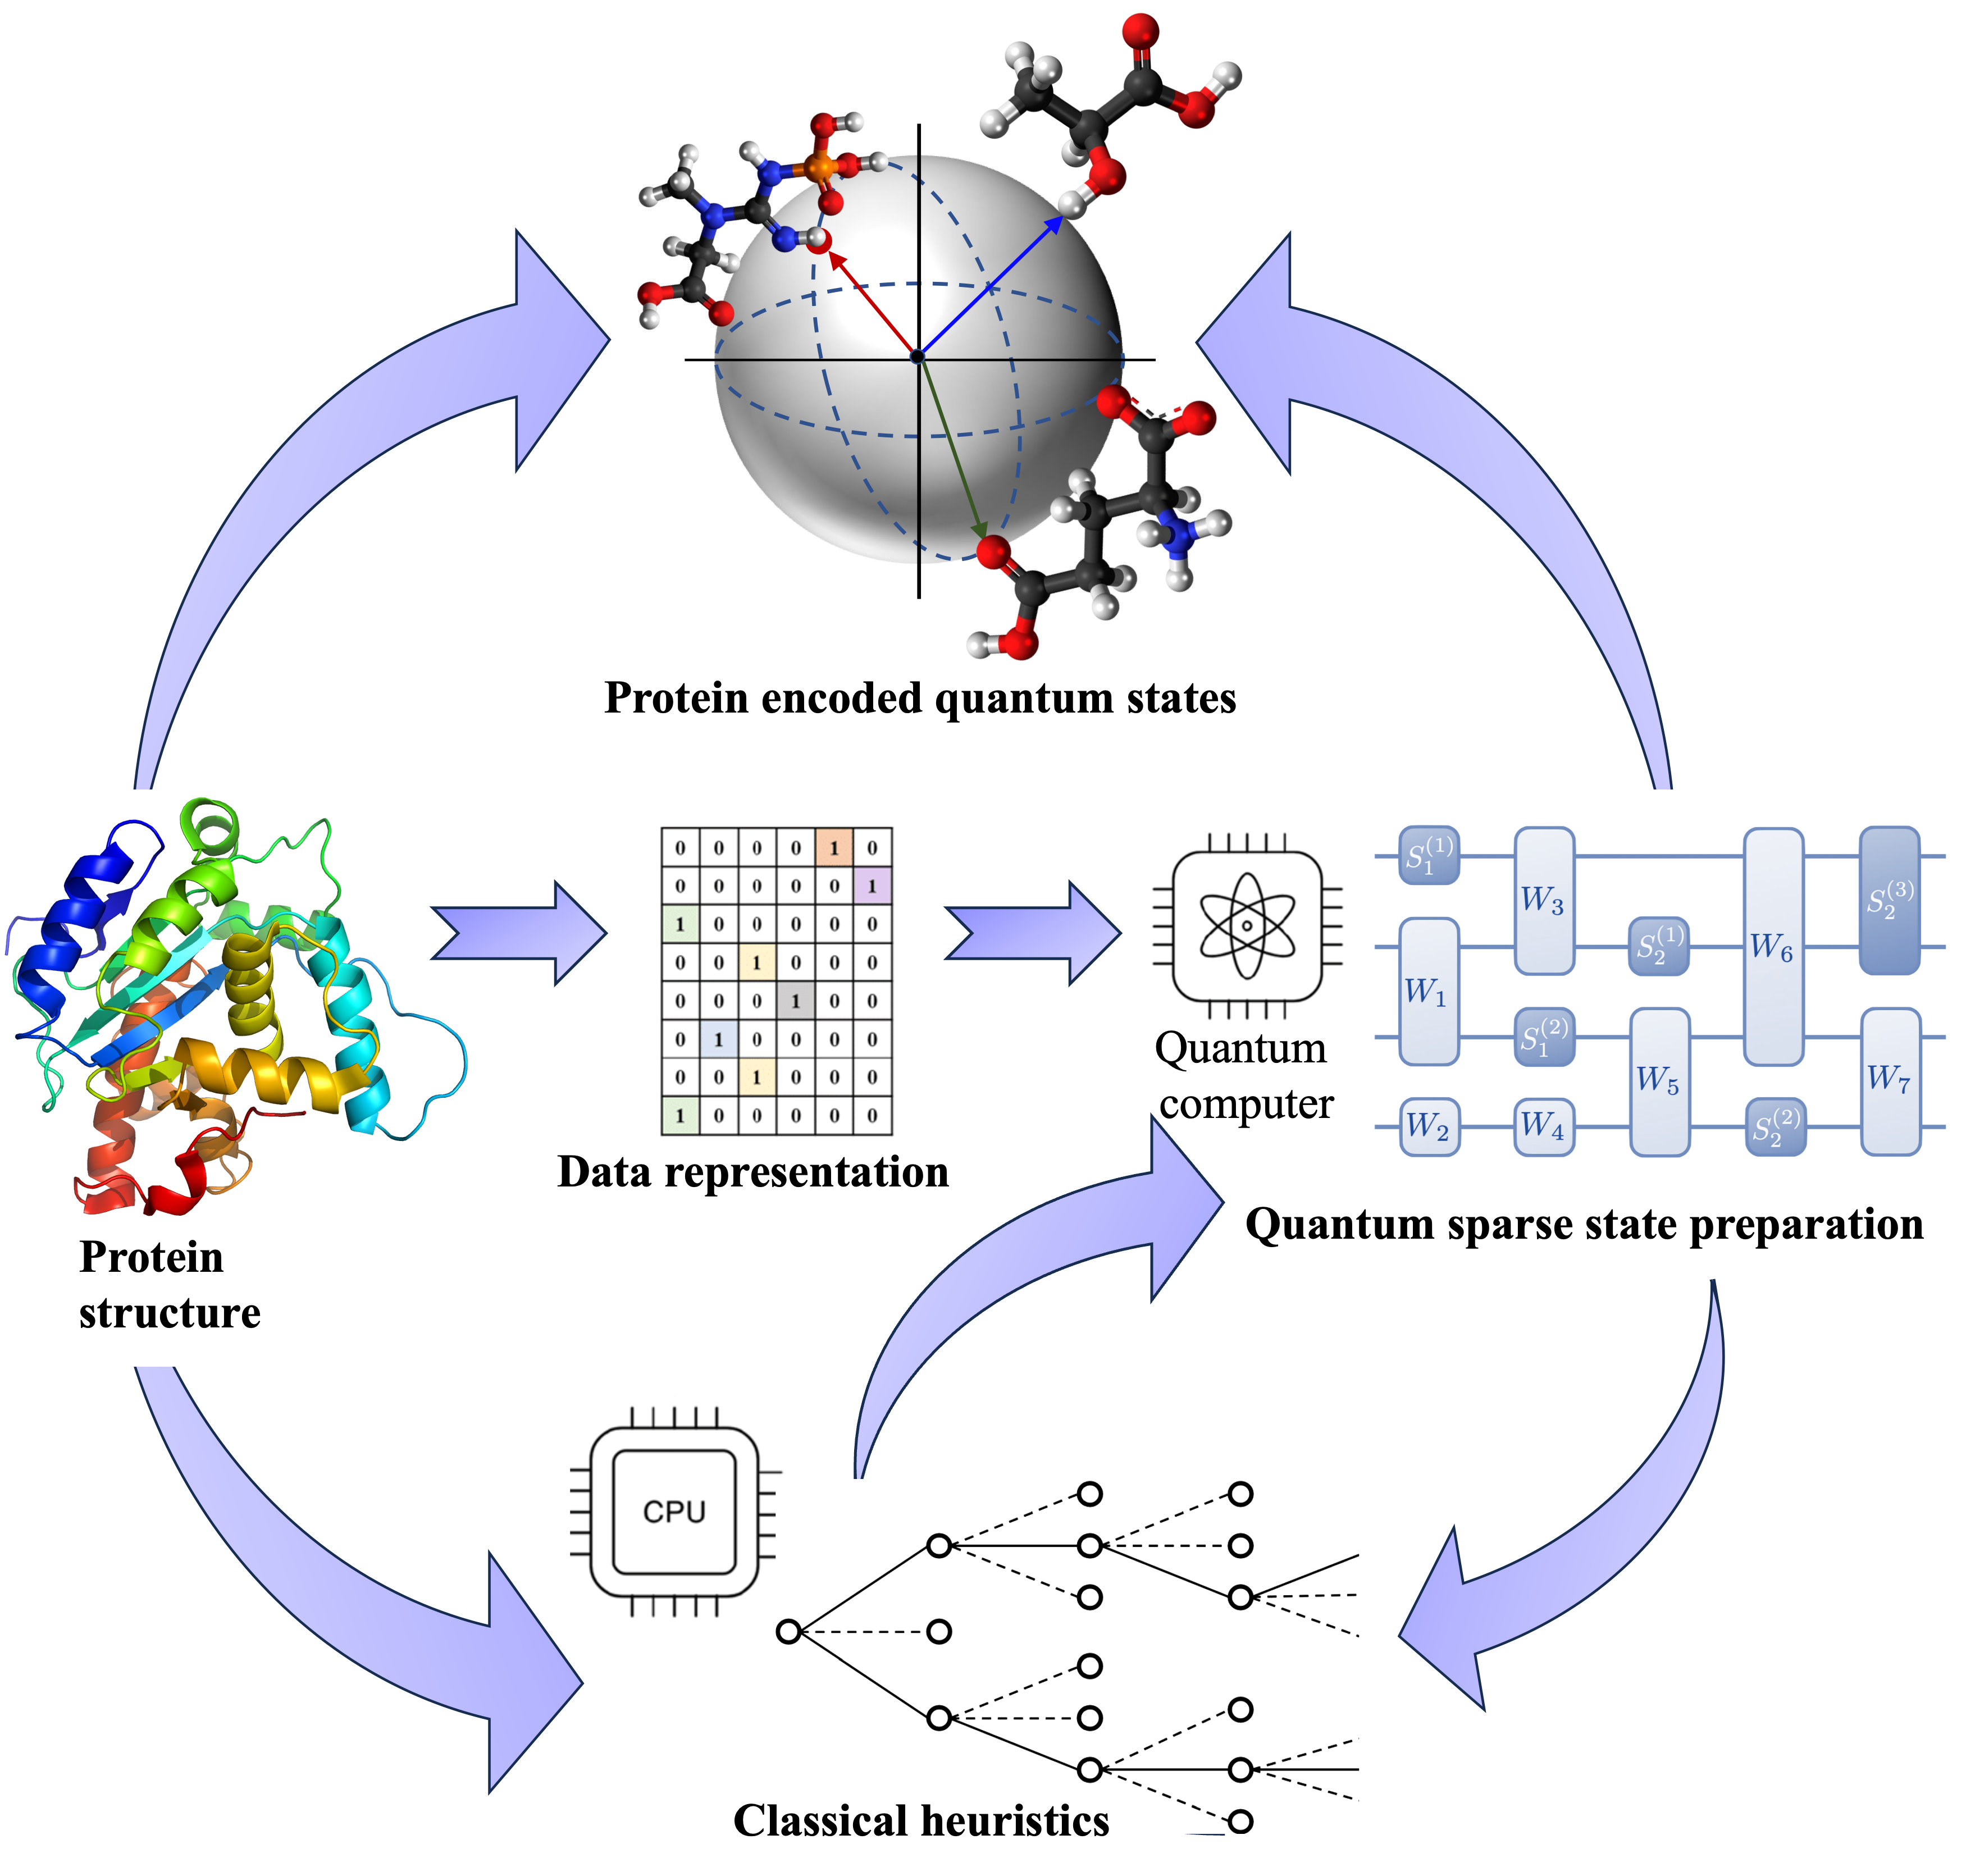
\includegraphics[width=1.0\linewidth]{main/figs/fig1.png}
\caption{An overview of the framework for encoding proteins as quantum states based on protein data representations, quantum sparse state preparation, and classical heuristics for refinement.}
\label{fig1}
\end{figure}

To instantiate the proposed framework, we address the problem of
preparing quantum states using fewer CX gates, but without using any
variational gate optimization procedure for computational efficiency. This
comes with three research challenges. The classical search heuristic finds
short gate sequences that approximately prepare quantum states with high fidelity. 
 The integration of the components within the proposed framework is achieved by iteratively applying the sparse QSP method which is hardware-adaptive. The proposed approach is implemented with the iterated sparse approximation (ISA) framework for LNN architectures. To show applicability to quantum states in both general and
machine learning applications, we apply our implementation to randomly sampled
quantum states up to 14 qubits and ten-qubit quantum states that encode proteins
from the UniProtKB database 
\cite{consortium2015uniprot}. We compared the CX gate count and classical
runtime of our ISA implementation against that of UCG and two VQC-based methods.
In addition, we studied the relationship between theoretical and observed 
preparation fidelity by performing noisy simulations of our algorithm on 
five-qubit states. The major contributions of this work are:
\begin{itemize}
  \item A novel, hardware-adaptive, non-variational framework for approximate 
  QSP is proposed.
  \item A connection between sparse QSP and general QSP is established
  \item A specific implementation of the proposed framework is described and
  shown to effectively prepare both generic quantum states and those
  representing real-world data.
\end{itemize}

% In section 2, we define the approximate QSP problem studied in this work. In 
% section 3, we describe the general ISA framework and our specific
% implementation. In section 4, we present three sets of experiments demonstrating
% the utility of our method. In section 5, we discuss the results and conclude. 
% Additional technical results are shown in the Appendix.